\documentclass[11pt,a4paper]{article}

\usepackage[T1]{fontenc}
\usepackage[utf8]{inputenc}
\usepackage{mathpazo}
\usepackage[margin=2.5cm]{geometry}
\usepackage{amsmath,amssymb,amsthm}
\usepackage{booktabs,array,tabularx}
\usepackage{graphicx}
\usepackage{xcolor}
\usepackage{titlesec}
\usepackage{enumitem}
\usepackage{tikz}
\usetikzlibrary{positioning,arrows.meta}
\usepackage{eso-pic}
\usepackage[most]{tcolorbox}
\usepackage[colorlinks=true,linkcolor=linkblue,citecolor=linkblue,urlcolor=linkblue]{hyperref}

% ---------- colours and headings (matching the school's report style) ----------
\definecolor{navy}{RGB}{31,42,94}
\definecolor{maroon}{RGB}{122,40,64}
\definecolor{boxblue}{RGB}{232,238,250}
\definecolor{boxedge}{RGB}{70,100,190}
\definecolor{linkblue}{RGB}{45,90,170}

\titleformat{\section}{\normalfont\fontsize{24}{28}\bfseries\color{navy}}{\thesection.}{0.6em}{}
\titlespacing*{\section}{0pt}{0pt}{18pt}
\titleformat{\subsection}{\normalfont\large\bfseries\color{maroon}}{}{0pt}{}
\titlespacing*{\subsection}{0pt}{14pt}{6pt}
\setlist[itemize]{leftmargin=1.6em,itemsep=2pt}

% page border on every page
\AddToShipoutPictureBG{%
  \begin{tikzpicture}[remember picture,overlay]
    \draw[line width=0.6pt] ([xshift=0.8cm,yshift=-0.8cm]current page.north west) rectangle ([xshift=-0.8cm,yshift=0.8cm]current page.south east);
  \end{tikzpicture}}

\newtheorem{proposition}{Proposition}

\tikzset{flowbox/.style={draw=boxedge,fill=boxblue,rounded corners=2pt,minimum width=11cm,minimum height=1.1cm,align=center,font=\small},
         arrow/.style={-{Stealth[length=2.5mm]},thick,color=black!70}}
\newcommand{\flowitem}[2]{\textbf{#1}\\#2}

\newtcolorbox{statementbox}{colback=boxblue,colframe=boxedge,boxrule=0.6pt,arc=2pt,fontupper=\itshape}

\begin{document}

% ================================ COVER ================================
\begin{titlepage}
\centering
\vspace*{2cm}

\includegraphics[width=0.62\textwidth]{figures/alliance_logo.png}\par
\vspace{1.2cm}
{\small ALLIANCE SCHOOL OF ADVANCED COMPUTING\par M. Tech. in Artificial Intelligence and Data Science\par}
\vspace{0.8cm}
{\bfseries Micro Project\par}
\vspace{1.4cm}
{\LARGE\bfseries Fuzzy RFM Formal Concept Analysis\\ for Customer Segmentation\par}
\vspace{0.3cm}
{\large\itshape Boundary-Aware, Describable and Stable Customer Segments\\ on Three Retail Datasets\par}
\vspace{1.4cm}
{\bfseries MICRO PROJECT REPORT\par}
\vspace{2cm}
\begin{tabular}{@{}ll@{}}
\textbf{Submitted by:} & Nandana Narayan Das \\
\textbf{Register No.:} & 2511022120032 \\
\textbf{Class:} & M. Tech. AI \& DS \\
\textbf{Course:} & % TODO: course name
[Course name] \\
\textbf{Guided by:} & % TODO: confirm guides
Tina Babu, Rekha R Nair \\
\textbf{University:} & Alliance University, Bengaluru \\
\end{tabular}
\vfill
\end{titlepage}

% ================================ ABSTRACT ================================
\section*{Abstract}
Customer segmentation with RFM (recency, frequency, monetary value) and formal concept analysis (FCA) gives segments that are explicitly described and arranged in a hierarchy. Its binary context, however, puts customers on either side of a quintile cut point into different segments although they behave almost the same. This micro project replaces the binary RFM context with a fuzzy one, in which a customer near a cut point belongs partly to both neighbouring quintiles, and builds segments from fuzzy formal concepts.

The project first replicates the crisp RFM-FCA method of Rungruang et al.\ (2024) on the UCI Online Retail II dataset, reproducing its 208 concepts and all 18 published rules. It then develops the fuzzy method, adding a \emph{core-support} threshold that removes uninformative concepts and a greedy 10-concept \emph{summary} for marketers, and evaluates it out of sample on three datasets (Online Retail II, CDNOW and dunnhumby) against the crisp method, a log-RFM model and K-means, Gaussian-mixture and fuzzy C-means clustering. Analysis plans were committed before each analysis.

Fuzzy RFM-FCA predicted next-period purchase and spend better than crisp RFM-FCA on all three datasets, a result that held in 47 of 48 settings of a sensitivity analysis. It reached 0.9--2.9 percentage points more revenue in the top customer decile and gave the most robust and stable segments of all methods compared. It was not a better predictor than log-RFM and was roughly level with fuzzy C-means, but unlike clustering its segments are exactly described by short rules, and it represents the 69--74\,\% of customers who lie near a quintile boundary.

\vspace{0.5em}
\noindent\textbf{Keywords:} customer segmentation, RFM, formal concept analysis, fuzzy logic, interpretability.

\newpage
\tableofcontents
\newpage

% ================================ 1 ================================
\section{Introduction}

Customer segmentation divides a customer base into groups that can be targeted with different marketing actions. Behavioural segmentation based on RFM, that is how recently a customer bought (recency), how often (frequency) and how much they spent (monetary value), is the most widely used approach in retail because it is cheap to compute, easy to explain and strongly predictive of future purchasing \cite{hughes1994,fader2005}.

Most RFM segmentations either group customers by quintile score combinations or cluster them with methods such as K-means \cite{chen2012}. Clusters, however, are described only by their centres and must be labelled by hand. Rungruang et al.\ \cite{rungruang2024} proposed using formal concept analysis (FCA) \cite{ganter1999}: the fifteen quintile indicators R1--R5, F1--F5 and M1--M5 form a binary table, and every segment is a \emph{formal concept} with an explicit description such as $\{R5, F5, M5\}$ (``very recent, very frequent, very high spending''). Concepts are ordered in a hierarchy and linked by association rules, which makes them directly usable by marketers.

The binary table has a weakness that the base paper itself lists as future work: a customer just below a quintile cut point and one just above it get different attributes, although their behaviour is almost the same. This project makes the table fuzzy and studies whether this gives better segments.

\subsection{Objectives}
\begin{itemize}
\item To replicate the crisp RFM-FCA method of Rungruang et al.\ on its own dataset.
\item To design a fuzzy RFM-FCA method in which customers near quintile boundaries belong partly to both neighbouring terms.
\item To make the fuzzy method practical: control the number of segments and provide a short summary for marketers.
\item To evaluate the method out of sample on three retail datasets against crisp RFM-FCA, log-RFM and standard clustering methods.
\item To assess prediction, targeting value, robustness, stability and interpretability of the segments.
\end{itemize}

\newpage
% ================================ 2 ================================
\section{Background and Literature Review}

\subsection{RFM segmentation}
RFM summarises a customer's purchase history in three numbers \cite{hughes1994}. Fader, Hardie and Lee \cite{fader2005} showed that RFM is a sufficient summary for predicting customer lifetime value under standard purchase models, using the CDNOW data that this project also uses. Chen, Sain and Guo \cite{chen2012} introduced the Online Retail data with an RFM and K-means case study. K-means, hierarchical clustering and Gaussian mixtures remain the usual segmentation methods \cite{wedel2000}.

\subsection{Fuzzy RFM}
Carrasco et al.\ \cite{carrasco2019} replaced crisp RFM scores by fuzzy linguistic values before K-means segmentation. Marín Díaz \cite{marindiaz2025} clustered RFM features with fuzzy C-means \cite{bezdek1981} and added explainable-AI post-processing. In both, the segments remain clusters: fuzziness softens the inputs or the assignment, but segments do not carry exact descriptions or an order between them.

\subsection{Formal concept analysis}
FCA builds a lattice of concepts (a set of objects together with the attributes they share) from a binary object--attribute table \cite{ganter1999}. It is widely used for knowledge discovery \cite{poelmans2013app,singh2016}. Large lattices are pruned by support or stability \cite{kuznetsov2007}, and rules are read along the lattice \cite{luxenburger1991}. Rungruang et al.\ \cite{rungruang2024} applied FCA to quintile RFM scores of Online Retail II customers and compared it with K-means and hierarchical clustering using cluster-validity indices.

\subsection{Fuzzy formal concept analysis}
Fuzzy FCA allows attributes to hold to a degree \cite{burusco1994,pollandt1997,belohlavek2002,belohlavek2004}. Surveys note that fuzzy lattices contain many more concepts, so concept reduction is essential in applications \cite{poelmans2014,alwersh2022}.

\subsection{Research gap}
Fuzzy formal concepts have not been used for RFM segmentation, and RFM-FCA has not been evaluated out of sample, against clustering baselines, or on more than one dataset. This project addresses all three.

\newpage
% ================================ 3 ================================
\section{Problem Identification}

The crisp RFM-FCA method gives readable segments, but several problems limit its use:

\begin{itemize}
\item \textbf{Hard boundaries.} 69--74\,\% of customers in the three datasets lie within 0.05 of a quintile cut point on at least one dimension. For them the crisp segment depends on a near-arbitrary line.
\item \textbf{Instability.} Because of these boundaries, a small change in the data can move many customers between segments.
\item \textbf{No out-of-sample evidence.} Segments were judged only by cluster indices on the same data, not by whether they predict what customers do next.
\item \textbf{One dataset.} All published results come from Online Retail II.
\item \textbf{Weak comparison.} Only K-means and hierarchical clustering were compared, with no simple RFM model as a benchmark.
\item \textbf{Concept explosion.} A naive fuzzy extension creates thousands of concepts (Section~\ref{sec:method}).
\end{itemize}

\subsection{Problem Statement}
\begin{statementbox}
To design a fuzzy RFM formal concept analysis method that represents customers near quintile boundaries, keeps the number of segments manageable, and is shown, by out-of-sample evaluation on several datasets, to give segments that are more predictive, more stable and as describable as those of crisp RFM-FCA and standard clustering.
\end{statementbox}

\newpage
% ================================ 4 ================================
\section{Existing System: Crisp RFM-FCA}

The base method \cite{rungruang2024} works as follows.

\begin{center}
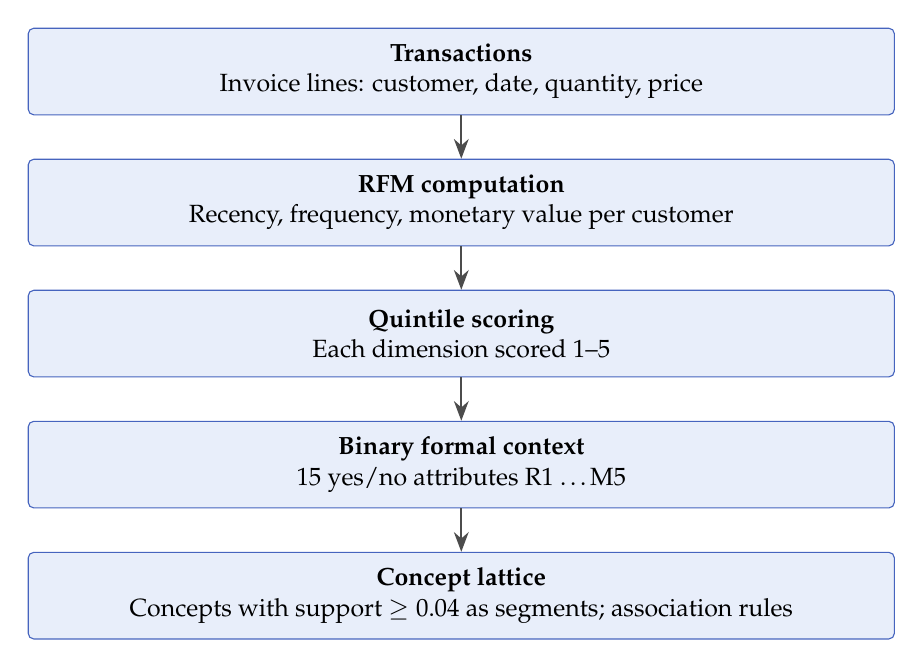
\begin{tikzpicture}[node distance=0.55cm]
\node[flowbox] (a) {\flowitem{Transactions}{Invoice lines: customer, date, quantity, price}};
\node[flowbox,below=of a] (b) {\flowitem{RFM computation}{Recency, frequency, monetary value per customer}};
\node[flowbox,below=of b] (c) {\flowitem{Quintile scoring}{Each dimension scored 1--5}};
\node[flowbox,below=of c] (d) {\flowitem{Binary formal context}{15 yes/no attributes R1 \dots M5}};
\node[flowbox,below=of d] (e) {\flowitem{Concept lattice}{Concepts with support $\ge 0.04$ as segments; association rules}};
\foreach \x/\y in {a/b,b/c,c/d,d/e} \draw[arrow] (\x) -- (\y);
\end{tikzpicture}\par
\small Figure 1: Crisp RFM-FCA pipeline of the base paper
\end{center}

\subsection{Limitations of the Existing Approach}
\begin{itemize}
\item \textbf{Binary membership:} a customer is either fully in a quintile or not, even right at a cut point.
\item \textbf{Boundary sensitivity:} small data changes flip customers between segments.
\item \textbf{Evaluation:} no test of predictive value, targeting value or stability.
\item \textbf{Single dataset:} generality unknown.
\end{itemize}

\newpage
% ================================ 5 ================================
\section{Dataset Description}

Three public or provider-supplied retail transaction datasets were used.

\begin{center}
\small
\begin{tabularx}{\textwidth}{@{}lXXX@{}}
\toprule
 & \textbf{Online Retail II} \cite{chen2019uci} & \textbf{CDNOW} \cite{fader2005} & \textbf{dunnhumby} \cite{dunnhumby} \\
\midrule
Domain & UK online gift wholesaler & Online music retailer & Grocery \\
Period & Dec 2009 -- Dec 2011 & Jan 1997 -- Jun 1998 & 711 days \\
Raw rows & 1,067,371 lines & 69,659 purchases & 2,595,732 basket lines \\
Customers & 5,878 (after cleaning) & 23,570 & 2,500 households \\
Special feature & Base paper's dataset & 52--65\,\% buy only once & 92--93\,\% buy in any 90 days \\
Role & Replication, development & Confirmation & Confirmation \\
\bottomrule
\end{tabularx}\par
\vspace{4pt}Table 1: Datasets used
\end{center}

\subsection{Pre-processing}
\begin{itemize}
\item Rows with missing customer IDs and non-positive quantities were removed; zero-price rows were kept, which reproduces the base paper's 805,620 cleaned lines.
\item For each customer and cutoff date: recency in calendar days since the last purchase, frequency as the number of transaction lines, and monetary value as total spend. Customers with zero total spend were dropped.
\item dunnhumby gives day numbers instead of dates; these were mapped to dates from an arbitrary anchor, since only differences between days matter.
\end{itemize}

\newpage
% ================================ 6 ================================
\section{Proposed Methodology}\label{sec:method}

\begin{center}
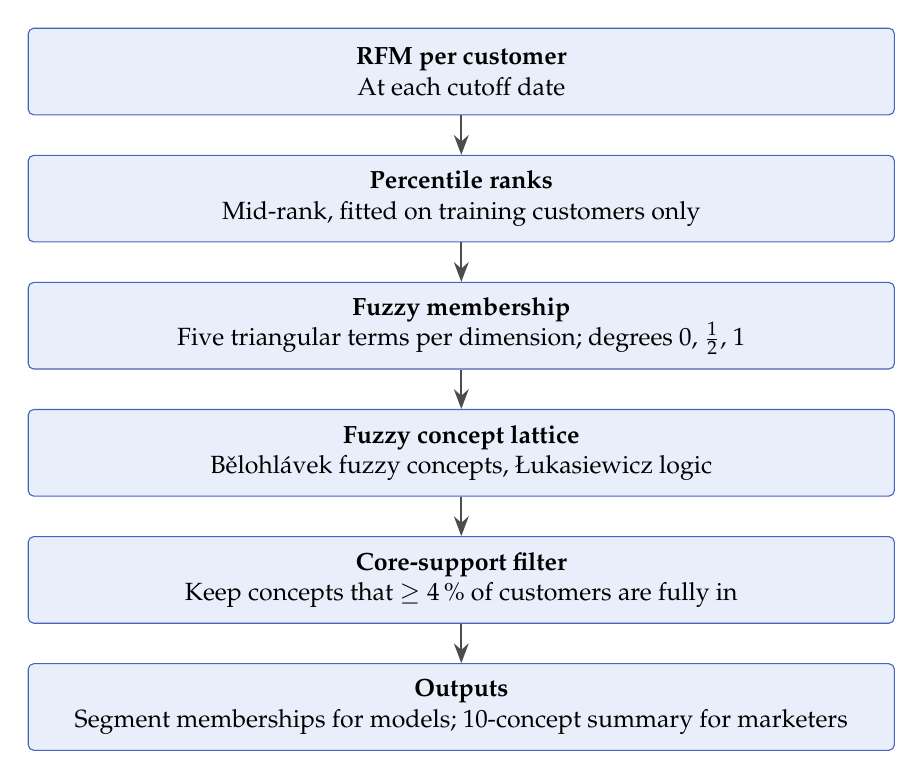
\begin{tikzpicture}[node distance=0.5cm]
\node[flowbox] (a) {\flowitem{RFM per customer}{At each cutoff date}};
\node[flowbox,below=of a] (b) {\flowitem{Percentile ranks}{Mid-rank, fitted on training customers only}};
\node[flowbox,below=of b] (c) {\flowitem{Fuzzy membership}{Five triangular terms per dimension; degrees 0, $\tfrac12$, 1}};
\node[flowbox,below=of c] (d) {\flowitem{Fuzzy concept lattice}{Bělohlávek fuzzy concepts, Łukasiewicz logic}};
\node[flowbox,below=of d] (e) {\flowitem{Core-support filter}{Keep concepts that $\ge 4\,\%$ of customers are fully in}};
\node[flowbox,below=of e] (f) {\flowitem{Outputs}{Segment memberships for models; 10-concept summary for marketers}};
\foreach \x/\y in {a/b,b/c,c/d,d/e,e/f} \draw[arrow] (\x) -- (\y);
\end{tikzpicture}\par
\small Figure 2: Proposed fuzzy RFM-FCA pipeline
\end{center}

\subsection{Fuzzy RFM context}
Each dimension is mapped to a percentile rank $u \in (0,1]$ (higher is better; recency reversed). Five triangular fuzzy sets are centred on the quintile midpoints $c_k = 0.1, 0.3, 0.5, 0.7, 0.9$ with half-width $0.2$:
\[
\mu_k(u) = \max\bigl(0,\ 1 - |u - c_k| / 0.2\bigr),
\]
with full membership at the two outer ends. The memberships of a customer add up to 1. A customer in the middle of a quintile band is fully in that term; one near a cut point is half in each neighbouring term. Degrees are rounded to $\{0, \tfrac12, 1\}$ (``not'', ``partly'', ``fully'').

\subsection{Fuzzy concepts and core support}
Segments are fuzzy formal concepts \cite{belohlavek2004}. A customer's degree of membership in a concept with description $B$ is $B^{\downarrow}(g) = \min_m \bigl(B(m) \to \tilde I(g,m)\bigr)$, where $\to$ is the Łukasiewicz implication $\min(1, 1-a+b)$. Under this logic every customer is at least half-way into any concept whose description contains only ``partly'' terms, so with the usual support threshold 2,649 of 3,841 concepts were kept on Online Retail II. The project therefore defines \textbf{core support}: the share of customers who are \emph{fully} in a concept. Concepts with core support of at least 0.04 become segments (208 on Online Retail II).

\subsection{Summary view}
For communication, 10 segments are chosen greedily so that each pick adds the most explained customer profile. No outcome data is used.

\subsection{Theoretical properties}
\begin{proposition}
Crisp RFM-FCA is a special case: the 0.5-cut of the fuzzy context is exactly the crisp quintile context, and with only the degrees $\{0,1\}$ the fuzzy lattice equals the crisp one.
\end{proposition}
\begin{proposition}
Core support does not depend on the fuzzy logic used, never increases when a description is extended, and equals ordinary support on binary data.
\end{proposition}
\begin{proposition}
The greedy summary is within $1 - 1/e \approx 63\,\%$ of the best possible summary of the same size \cite{nemhauser1978}.
\end{proposition}
Proofs are given in the accompanying paper, and all propositions are checked numerically in the project's test suite.

\newpage
% ================================ 7 ================================
\section{Implementation}

\subsection{Tools}
\begin{itemize}
\item \textbf{Language:} Python 3, with pandas and NumPy for data handling.
\item \textbf{Fuzzy FCA:} implemented from scratch (concept lattice by meet-closure, Łukasiewicz and Gödel logic, core support, greedy summary).
\item \textbf{Models and baselines:} scikit-learn \cite{pedregosa2011} for logistic and ridge regression, K-means and Gaussian mixtures; fuzzy C-means implemented and unit-tested.
\item \textbf{Testing:} pytest suite of 30 tests, including numerical checks of the theory.
\item \textbf{Reproducibility:} all code, analysis plans and results in a public Git repository.
\end{itemize}

\subsection{Evaluation protocol}
\begin{itemize}
\item \textbf{Rolling origin} \cite{tashman2000}: four cutoff dates per dataset; features from the history before each cutoff, targets from the next 90 days.
\item \textbf{Targets:} whether a customer buys (ROC AUC, logistic regression) and log spend ($R^2$, ridge regression).
\item \textbf{Cross-validation:} 5 folds per cutoff; ranks, lattices, summaries and clusters fitted on training customers only.
\item \textbf{Statistics:} paired customer bootstrap with 1,000 resamples \cite{efron1993}, Holm correction for multiple tests \cite{holm1979}.
\item \textbf{Pre-registration:} an analysis plan and eleven addenda were committed before each analysis. The method was developed on Online Retail II and confirmed on CDNOW and dunnhumby without changes.
\end{itemize}

\subsection{Methods compared}
\begin{center}
\small
\begin{tabular}{@{}lll@{}}
\toprule
Code & Description & Role \\
\midrule
C-ctx & 15 crisp quintile indicators & ablation \\
C-fca & crisp concept lattice \cite{rungruang2024} & base method \\
F-ctx & 15 fuzzy memberships & ablation \\
F-fca-core & fuzzy concept lattice, core support & proposed \\
log-RFM & log of R, F, M & benchmark \\
KM, GMM, FCM & K-means, Gaussian mixture, fuzzy C-means ($k = 10$) & baselines \\
\bottomrule
\end{tabular}\par
\vspace{4pt}Table 2: Representations compared
\end{center}

\newpage
% ================================ 8 ================================
\section{Results and Discussion}

\subsection{Replication of the base paper}
The crisp implementation reproduced the base paper on Online Retail II: 805,620 cleaned lines, 5,878 customers and 208 formal concepts, as published. The 34 printed concept sizes were matched to within 0.8 customers on average, and all 18 published rules were recomputed with confidences within 0.01.

\subsection{Development and confirmation}
The first fuzzy version used the usual support threshold and failed (AUC 0.733 vs 0.781 for crisp), which led to core support. With core support, the method was tested unchanged on the other two datasets: on CDNOW all seven pre-registered claims replicated; on dunnhumby four did, while two claims (the lattice adding spend signal beyond the fuzzy memberships, and robustness to dropped transactions) did not and are therefore not claimed.

\subsection{Prediction}
\begin{table}[t]
\centering\small
\caption{Out-of-sample prediction of the next 90 days (means over four cutoffs; regularisation tuned by inner cross-validation). Best value per column in bold.}
\label{tab:prediction}
\begin{tabular}{lcccccc}
\toprule
 & \multicolumn{3}{c}{ROC AUC (purchase)} & \multicolumn{3}{c}{$R^2$ (log spend)} \\
\cmidrule(lr){2-4}\cmidrule(lr){5-7}
Representation & Retail II & CDNOW & dunnhumby & Retail II & CDNOW & dunnhumby \\
\midrule
Crisp scores (C-ctx) & 0.782 & 0.784 & 0.869 & 0.296 & 0.209 & 0.511 \\
Crisp RFM-FCA (C-fca) & 0.780 & 0.784 & 0.855 & 0.299 & 0.222 & 0.508 \\
Fuzzy memberships (F-ctx) & \textbf{0.787} & \textbf{0.789} & 0.877 & 0.304 & 0.219 & \textbf{0.525} \\
Fuzzy RFM-FCA (F-fca-core) & 0.786 & 0.788 & 0.865 & \textbf{0.308} & 0.235 & 0.517 \\
log-RFM & 0.786 & 0.788 & \textbf{0.887} & 0.293 & \textbf{0.241} & 0.517 \\
K-means, $k{=}10$ & 0.764 & 0.777 & 0.828 & 0.289 & 0.236 & 0.498 \\
GMM, $k{=}10$ & 0.770 & 0.778 & 0.875 & 0.260 & 0.232 & 0.453 \\
FCM, $k{=}10$ & 0.783 & 0.786 & 0.860 & 0.290 & 0.239 & 0.511 \\
\bottomrule
\end{tabular}
\end{table}

\begin{table}[t]
\centering\small
\caption{Paired differences (first minus second representation), tuned regularisation, pooled over four cutoffs. $^{*}$: 95\,\% customer-bootstrap interval excludes zero.}
\label{tab:comparisons}
\begin{tabular}{lcccccc}
\toprule
 & \multicolumn{3}{c}{$\Delta$ AUC} & \multicolumn{3}{c}{$\Delta R^2$} \\
\cmidrule(lr){2-4}\cmidrule(lr){5-7}
Comparison & Retail II & CDNOW & dunnhumby & Retail II & CDNOW & dunnhumby \\
\midrule
Fuzzification (memberships) & +0.0048$^{*}$ & +0.0048$^{*}$ & +0.0076$^{*}$ & +0.0080$^{*}$ & +0.0099$^{*}$ & +0.0141$^{*}$ \\
Fuzzy vs crisp RFM-FCA & +0.0063$^{*}$ & +0.0040$^{*}$ & +0.0098$^{*}$ & +0.0089$^{*}$ & +0.0124$^{*}$ & +0.0089$^{*}$ \\
Lattice beyond memberships & -0.0008 & -0.0007 & -0.0117$^{*}$ & +0.0044$^{*}$ & +0.0154$^{*}$ & -0.0082$^{*}$ \\
vs K-means, $k{=}10$ & +0.0220$^{*}$ & +0.0111$^{*}$ & +0.0372$^{*}$ & +0.0189$^{*}$ & -0.0017 & +0.0186$^{*}$ \\
vs GMM, $k{=}10$ & +0.0163$^{*}$ & +0.0102$^{*}$ & -0.0101$^{*}$ & +0.0487$^{*}$ & +0.0024 & +0.0634$^{*}$ \\
vs FCM, $k{=}10$ & +0.0029$^{*}$ & +0.0021$^{*}$ & +0.0052 & +0.0180$^{*}$ & -0.0047$^{*}$ & +0.0058 \\
\bottomrule
\end{tabular}
\end{table}

Fuzzy RFM-FCA beat crisp RFM-FCA on all three datasets (0.004--0.010 AUC, 0.009--0.012 $R^2$), and fuzzy memberships beat crisp scores. It beat K-means in five of six cells and the Gaussian mixture in four, and was roughly level with fuzzy C-means. No segmentation beat log-RFM, which keeps the exact values that segments compress.

\subsection{Targeting value}
\begin{table}[t]
\centering\small
\caption{Share of next-90-day revenue (\%) held by the top 10\,\% and 20\,\% of customers ranked by predicted spend (means over four cutoffs).}
\label{tab:targeting}
\begin{tabular}{lcccccc}
\toprule
 & \multicolumn{3}{c}{Top 10\,\%} & \multicolumn{3}{c}{Top 20\,\%} \\
\cmidrule(lr){2-4}\cmidrule(lr){5-7}
Representation & Retail II & CDNOW & dunnhumby & Retail II & CDNOW & dunnhumby \\
\midrule
Crisp RFM-FCA (C-fca) & 52.6 & 52.6 & 28.3 & 71.6 & 70.6 & 50.1 \\
Fuzzy RFM-FCA (F-fca-core) & 55.4 & 53.5 & 30.5 & 71.8 & 70.4 & 50.7 \\
Fuzzy memberships (F-ctx) & 55.6 & 52.8 & 30.6 & 73.4 & 70.1 & 50.9 \\
log-RFM & 58.0 & 52.8 & 31.2 & 72.3 & 69.9 & 50.0 \\
K-means, $k{=}10$ & 54.1 & 51.6 & 28.6 & 70.3 & 68.7 & 48.3 \\
GMM, $k{=}10$ & 51.2 & 51.2 & 21.7 & 70.1 & 68.0 & 38.7 \\
FCM, $k{=}10$ & 36.2 & 53.8 & 26.8 & 71.2 & 70.2 & 49.5 \\
\bottomrule
\end{tabular}
\end{table}

\begin{figure}[t]
\centering
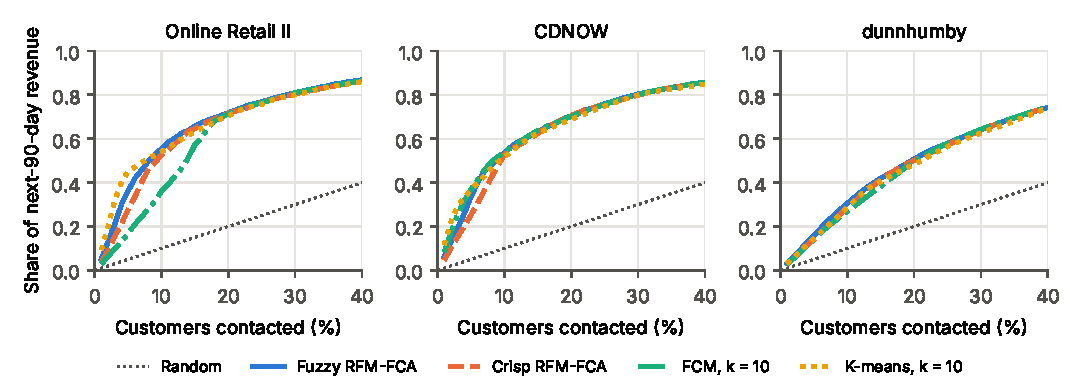
\includegraphics[width=\textwidth]{figures/gain_curves.pdf}
\caption{Share of next-90-day revenue reached against the share of customers contacted.}
\label{fig:gain}
\end{figure}
Contacting the top 10\,\% of customers ranked by fuzzy RFM-FCA reached 0.9--2.9 percentage points more revenue than ranking by crisp RFM-FCA on every dataset (Table~\ref{tab:targeting}, Figure~\ref{fig:gain}).

\subsection{Robustness and stability}
\begin{table}[t]
\centering\small
\caption{Structural agreement (correlation of customer-pair similarities between a reference fit and a perturbed fit; 1 = identical), mean over 20 replicates. Robustness: 5\,\% of invoices dropped. Stability: bootstrap resample of customers.}
\label{tab:structure}
\begin{tabular}{lcccccc}
\toprule
 & \multicolumn{3}{c}{Robustness} & \multicolumn{3}{c}{Stability} \\
\cmidrule(lr){2-4}\cmidrule(lr){5-7}
Representation & Retail II & CDNOW & dunnhumby & Retail II & CDNOW & dunnhumby \\
\midrule
Crisp RFM-FCA (C-fca) & 0.886 & 0.936 & 0.928 & 0.957 & 0.987 & 0.936 \\
Fuzzy RFM-FCA (F-fca-core) & 0.958 & 0.955 & 0.948 & 0.986 & 0.993 & 0.972 \\
K-means, $k{=}10$ & 0.760 & 0.907 & 0.650 & 0.683 & 0.937 & 0.692 \\
GMM, $k{=}10$ & 0.858 & 0.816 & 0.878 & 0.818 & 0.904 & 0.843 \\
FCM, $k{=}10$ & 0.913 & 0.929 & 0.942 & 0.944 & 0.966 & 0.914 \\
\bottomrule
\end{tabular}
\end{table}

Fuzzy RFM-FCA had the highest mean robustness and stability of all methods on all three datasets (Table~\ref{tab:structure}).

\subsection{Interpretability and the summary view}
\begin{table}[t]
\centering\small
\caption{Structural interpretability proxies on the full data (Retail II / CDNOW / dunnhumby). Fidelity: F1 between ``satisfies the segment's R/F/M description'' and ``is a member''. Conditions: constrained dimensions per description.}
\label{tab:interpretability}
\begin{tabular}{lcccc}
\toprule
Representation & Segments & Fidelity (F1) & Conditions & Segments per customer \\
\midrule
Crisp RFM-FCA (C-fca) & 51 / 54 / 49 & 1.00 / 1.00 / 1.00 & 1.5 / 1.6 / 1.5 & 5.3 / 6.2 / 5.5 \\
Fuzzy RFM-FCA (F-fca-core) & 208 / 238 / 215 & 1.00 / 1.00 / 1.00 & 1.8 / 1.9 / 1.8 & 19.5 / 24.0 / 20.9 \\
K-means, $k{=}10$ & 10 / 10 / 10 & 0.68 / 0.74 / 0.74 & 3.0 / 3.0 / 3.0 & 1.0 / 1.0 / 1.0 \\
GMM, $k{=}10$ & 10 / 10 / 10 & 0.53 / 0.80 / 0.67 & 3.0 / 3.0 / 3.0 & 1.0 / 1.0 / 1.0 \\
FCM, $k{=}10$ & 10 / 10 / 10 & 0.66 / 0.71 / 0.73 & 3.0 / 3.0 / 3.0 & 1.0 / 1.0 / 1.0 \\
\bottomrule
\end{tabular}
\end{table}

\begin{table}[t]
\centering\small
\caption{The 10-concept fuzzy summary of Online Retail II (greedy description-coverage selection, full data). $\tfrac12$X: partly in term X.}
\label{tab:summaryview}
\begin{tabular}{rlrr}
\toprule
\# & Intent & Customers fully in (\%) & Share of spend (\%) \\
\midrule
1 & \{F5, M5\} & 10.3 & 55.3 \\
2 & \{F1, M1\} & 9.9 & 0.4 \\
3 & \{$\tfrac12$F2, $\tfrac12$M2\} & 18.9 & 2.7 \\
4 & \{$\tfrac12$F4, $\tfrac12$M4\} & 18.8 & 13.0 \\
5 & \{$\tfrac12$F3, $\tfrac12$M3\} & 17.9 & 5.6 \\
6 & \{$\tfrac12$F2, M1\} & 4.6 & 0.2 \\
7 & \{F5, $\tfrac12$M4\} & 4.5 & 3.6 \\
8 & \{$\tfrac12$F4, $\tfrac12$F5, $\tfrac12$M5\} & 6.3 & 11.8 \\
9 & \{$\tfrac12$F1, $\tfrac12$M1, $\tfrac12$M2\} & 6.2 & 0.6 \\
10 & \{R5, F5, M5\} & 4.8 & 36.9 \\
\bottomrule
\end{tabular}
\end{table}

FCA segments are exactly described by their intents in fewer than two conditions, while the best R/F/M description of a cluster disagrees with its membership for 20--47\,\% of customers (Table~\ref{tab:interpretability}). The full fuzzy lattice has about four times as many segments as the crisp one; the 10-concept summary (Table~\ref{tab:summaryview}) fixes this, with each customer in one or two segments. It beats the crisp 10-concept summary on prediction and stability, but predicts worse than fuzzy C-means with ten clusters.

\subsection{Sensitivity analysis}
\begin{table}[t]
\centering\small
\caption{Sensitivity analysis: number of setting $\times$ dataset $\times$ metric cells in which the fuzzy variant is significantly better (95\,\% interval above zero) and significantly worse. Settings: support 0.02/0.04/0.06, membership half-width 0.15/0.20/0.25, horizon 60/90/180 days.}
\label{tab:sensitivity}
\begin{tabular}{lcc}
\toprule
Comparison & Fuzzy significantly better & Significantly worse \\
\midrule
Fuzzy vs crisp RFM-FCA & 47 / 48 & 0 \\
Fuzzy vs crisp memberships & 29 / 30 & 1 \\
Fuzzy vs crisp summary ($K = 5, 10, 20, 30$) & 18 / 24 & 1 \\
\bottomrule
\end{tabular}
\end{table}

\begin{figure}[t]
\centering
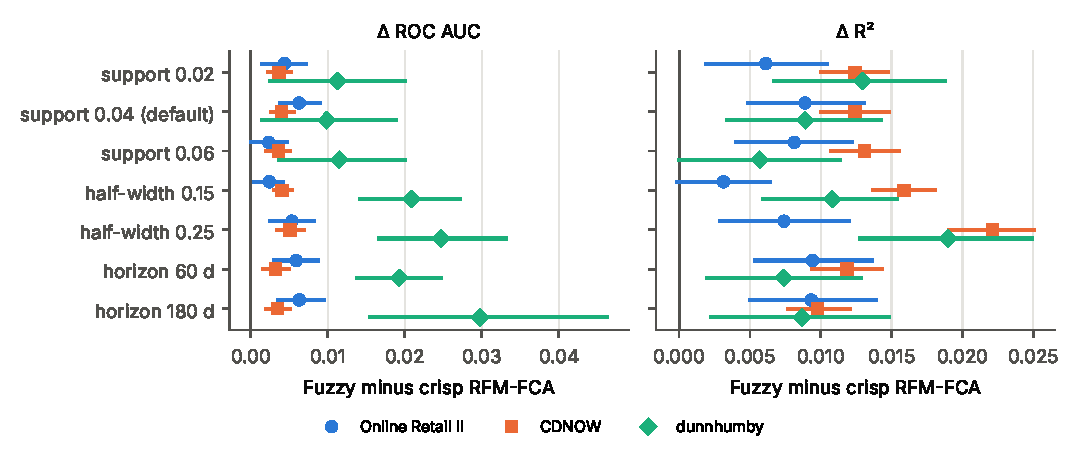
\includegraphics[width=\textwidth]{figures/sensitivity.pdf}
\caption{Fuzzy minus crisp RFM-FCA under one-at-a-time parameter changes, with 95\,\% intervals.}
\label{fig:sens}
\end{figure}
Varying the support threshold, membership width and prediction horizon, fuzzy RFM-FCA beat crisp RFM-FCA significantly in 47 of 48 cases and was never worse (Table~\ref{tab:sensitivity}, Figure~\ref{fig:sens}).

\newpage
% ================================ 9 ================================
\section{Findings}
\begin{itemize}
\item Fuzzy RFM-FCA predicts next-period purchase and spend better than crisp RFM-FCA on all three datasets.
\item The result does not depend on the parameters chosen: 47 of 48 sensitivity settings, none worse.
\item It reaches 0.9--2.9 percentage points more revenue in the top 10\,\% of customers.
\item It gives the most robust and stable segments of all methods compared.
\item Like crisp FCA and unlike clustering, its segments are exactly described by short rules.
\item It is not a better predictor than log-RFM and is roughly level with fuzzy C-means.
\item A 10-concept summary makes the segments readable for marketers.
\end{itemize}

\section{Challenges and Limitations}
\begin{itemize}
\item \textbf{Concept explosion:} the naive fuzzy lattice kept 2,649 concepts; solved with core support.
\item \textbf{Small effects:} gains over crisp RFM-FCA are 0.004--0.010 AUC.
\item \textbf{Regularisation:} on smaller datasets the fuzzy lattice needs tuned regularisation.
\item \textbf{Interpretability:} measured with structural proxies, not with marketers.
\item \textbf{Ties:} heavily tied frequencies (CDNOW) reduce the benefit of fuzzy memberships; an exploratory tie-aware variant addresses this.
\item \textbf{Scope:} only retail data and a three-level truth scale were studied.
\end{itemize}

\section{Future Scope}
\begin{itemize}
\item A user study with marketers to test whether fuzzy segments are more useful in practice.
\item Five-level truth scales and other membership shapes.
\item Confirmation of the tie-aware variant on a dataset with many one-time buyers.
\item Applications outside retail, e.g.\ banking and telecom.
\item A dashboard presenting the 10-concept summary and its rules to marketing teams.
\end{itemize}

\section{Conclusion}
This micro project extended RFM segmentation with formal concept analysis from a binary to a fuzzy context. After replicating the base method, it developed a fuzzy RFM-FCA with a core-support threshold and a 10-concept summary, and evaluated it out of sample on three retail datasets with pre-registered analyses. Fuzzy RFM-FCA beat crisp RFM-FCA on prediction, top-decile targeting, robustness and stability, a result that held in 47 of 48 sensitivity settings, and it beat K-means and was roughly level with fuzzy C-means while providing segments with exact rule descriptions. It is not a better predictor than log-RFM; its value lies in segments that are boundary-aware, stable and directly describable.

\vspace{1em}
\noindent\textbf{Code and data:} \url{https://github.com/nandana-das/rfm-fuzzy}

\bibliographystyle{unsrt}
\bibliography{refs}

\end{document}
